\title{Latches and Flip-Flops}
\begin{document}
\section{The Bistable Circuit}

\begin{frame}{Sequential circuits}
  \begin{definition}
    A \alert{sequential circuit} is a digital circuit which defines outputs that depend on its current and previous inputs.
  \end{definition}
  Sequential circuits often use a \alert{clock signal} to determine when inputs will be applied.
\end{frame}

\begin{frame}{Yes, Viginia, this is a real digital circuit}
  \begin{block}{Does a circuit with no inputs make sense?}
    The \alert{bistable} circuit is a digital circuit consisting of no inputs, two outputs, and two inverters.
  \end{block}
  \begin{center}
    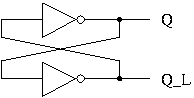
\includegraphics{BistableCircuit}
  \end{center}
  \begin{itemize}
    \item This circuit does have some applications, which we'll discuss later.
    \item We explore this circuit is to understand its transient (\alert{metastable}) behavior.
    \item This is like the bowling ball game at the fair.
  \end{itemize}
\end{frame}

\section{S-R Latches}

\begin{frame}{Boring (but important) terminoloy note}
  \begin{definition}
    A \alert{latch} is a sequential circuit that watches its inputs continuously and can change its outputs at any time.
  \end{definition}
  \begin{definition}
    A \alert{flip-flop} is a sequential circuit that changes its outputs only when a clocking signal is changed.
  \end{definition}
\end{frame}

\subsection{S-R Latches}

\begin{frame}{The S-R (set-reset) latch}
  \begin{columns}
    \begin{column}{6cm}
      \begin{center}
        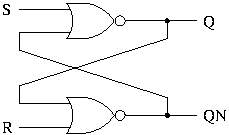
\includegraphics{SRLatchCircuit}
      \end{center}
    \end{column}
    \begin{column}{6cm}
      \begin{center}
        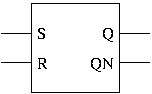
\includegraphics{SRLatchSchematicActiveHigh} \\
      \end{center}
      \begin{center}
        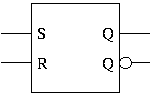
\includegraphics{SRLatchSchematicActiveLow} \\
      \end{center}
    \end{column}
  \end{columns}
  \begin{itemize}
    \item The S input sets or presets the output Q to 1.
    \item The R input resets or clears the output Q to 0.
    \item A \alert{minimum pulse width} for S and R specifies how long they must be asserted to avoid the metastable behavior.
  \end{itemize}
\end{frame}

Do function table.

\subsection{$\bar{S}-\bar{R}$ Latch}

\begin{frame}{$\bar{S}-\bar{R}$ Latch}
  \begin{columns}
    \begin{column}{6cm}
      \begin{center}
        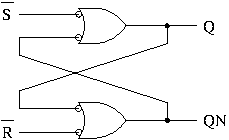
\includegraphics{SbarRbarLatchCircuit}
      \end{center}
    \end{column}
    \begin{column}{6cm}
      \begin{center}
        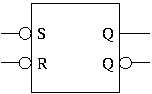
\includegraphics{SbarRbarLatchSchematic}
      \end{center}
    \end{column}
  \end{columns}
\end{frame}

Do function table.

\subsection{S-R Latch with Enable}

\begin{frame}{S-R Latch with Enable}
  \begin{columns}
    \begin{column}{6cm}
      \begin{center}
        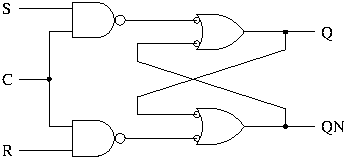
\includegraphics{SRLatchWithEnableCircuit}
      \end{center}
    \end{column}
    \begin{column}{6cm}
      \begin{center}
        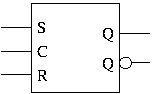
\includegraphics{SRLatchWithEnableSchematic}
      \end{center}
    \end{column}
  \end{columns}
\end{frame}

Do function table.

\section{D Latches and Flip-Flops}

\subsection{D Latch}

\begin{frame}{D Latch}
  \begin{columns}
    \begin{column}{6cm}
      \begin{center}
        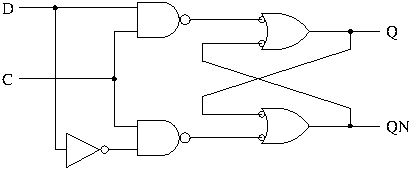
\includegraphics{DLatchCircuit}
      \end{center}
    \end{column}
    \begin{column}{6cm}
      \begin{center}
        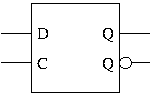
\includegraphics{DLatchSchematic}
      \end{center}
    \end{column}
  \end{columns}
\end{frame}

Do function table.

\subsection{D Flip-Flop}

\begin{frame}{D flip-flop}
  \begin{center}
    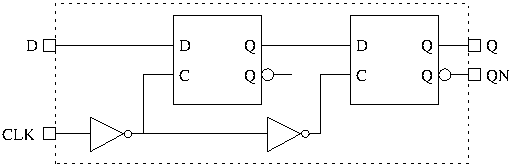
\includegraphics{DFlipFlopLogic} \\
    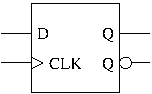
\includegraphics{DFlipFlopSchematic}
  \end{center}
\end{frame}

\begin{itemize}
  \item We can also have a D flip-flop that works on the falling clock edge.
  \item Some D flip-flops have PR(preset) and CLR (clear) inputs that are used to initialization.
  \item Note that usually, D flip-flops are not implemented using two D Latches.  See Fig 7-20 on page 535.
\end{itemize}

\subsection{D Flip-Flop with Enable}

\begin{frame}{D flip-flop with enable}
  \begin{center}
    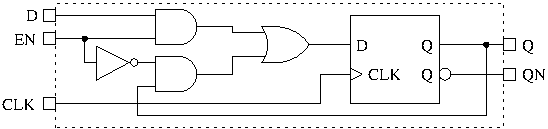
\includegraphics{DFlipFlopLogicWithEnable} \\
    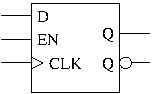
\includegraphics{DFlipFlopSchematicWithEnable}
  \end{center}
\end{frame}

\section{T Flip-Flop}
\begin{frame}{T flip-flop with enable}
  \begin{center}
    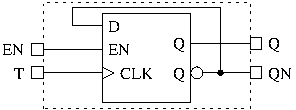
\includegraphics{TFlipFlopLogic} \\
    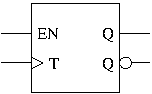
\includegraphics{TFlipFlopSchematic}
  \end{center}
\end{frame}

\end{document}
